\chapter{Ergebnisse}
\label{ch:results}

In diesem Kapitel werden die Ergebnisse der in \autoref{sec:experimente} beschriebenen Experimente vorgestellt.
Die Evaluation schließt die Ergebnisse aller vier Phasen, häufige Fehler in der Verifikation, sowie eine grobe Kategorisierung der Aktionsklassen ein.

\section{Benchmark}
\label{sec:benchmark}

In diesem Abschnitt werden die Rechenergebnisse der verschiedenen Modelle miteinander verglichen.
Als Baseline-Modelle wurden R2+1D-34, ir-CSN-152 und zwei Varianten von SlowFast-50 getestet, die mit $\gls{tld:Theta}_\text{train} = 200$ für 10 Epochen trainiert.
Beide SlowFast-Varianten wurden zunächst ohne Hinzunahme von Non-Local-Blöcken trainiert.
In \autoref{tab:phase1} sind die Ergebnisse zu sehen, wobei alle Hyperparameter aus den ursprünglichen Publikationen übernommen wurden.
Die Metriken basieren auf einem einheitlichen Testset mit $\Delta_\text{test} = 3$.
Der Zeitkontext im Testset ist damit größer als im Trainingsset und wird durch zusätzliche Frames erreicht (\zB 36 statt 32 Frames bei ir-CSN), die die Modelle durch ihr dynamisches Pooling wieder auf die passende Länge stauchen.

Überraschend ist, dass die SlowFast-Variante mit $\alpha = 8$ (SlowFast-50-4x16) bessere Ergebnisse erzielt als die Variante mit $\alpha = 4$ (SlowFast-50-8x8).
Im ersteren erhält der Slow-Pathway schließlich nur halb so viele Frames, wie im letzteren und kann sich damit noch mehr auf räumliche Features fokussieren.
Da die Ergebnisse für SlowFast-50-4x16 durchweg besser ausfallen, wird diese Variante im weiteren Verlauf als SlowFast-Baseline-Modell bezeichnet.

\begin{figure}
    \centering
    \small
    \csvreader[no head,tabular=|l|r||r|r|r|r|,
    table head=\hline,late after line=\\\hline]{tbl/exp_phase_1.csv}
    {1=\model,2=\aurocval,3=\baval,4=\fbetaval,5=\lr,6=\bs,7=\ba,8=\rec,9=\prec,10=\auroc}
    {\model & \lr & \ba & \prec & \rec & \auroc}
    \caption{Ergebnisse aus Benchmark}
    \label{tab:phase1}
\end{figure}

\subsection{Vergleich der Modelle}
\label{subsec:vergleich-der-modelle}

Vergleicht man die Ergebnisse, fällt auf, dass ir-CSN die besten und R2+1D die schwächsten Metriken vorweist.
Damit einher geht allerdings auch ein größerer Fußabdruck:
während bei R2+1D (\bzw SlowFast) eine maximale Batch-Größe von 24 (\bzw 21) möglich war, erlaubt ir-CSN nur eine Batch-Größe von maximal 5 bei gleicher Speicherauslastung.
Dennoch wird für den weiteren Verlauf ir-CSN als einziges Baseline-Modell weitergeführt.
Die weitere Optimierung der anderen Modelle wird aus Zeitgründen nicht weiter verfolgt.

\subsection{Verifikation}
\label{sec:verifikation}

Im nächsten Schritt werden die Fehler der Experimente genauer analysiert.
Grundlage sind die drei Baseline-Modelle aus der ersten Phase.
Im Zuge der Analyse werden innerhalb einer statistischen Analyse Auffälligkeiten im Fehlerreport analysiert.
Zusätzlich werden jeweils 50 der Samples mit den größten Fehlerwerten innerhalb eines Experiments verifiziert.

Bei der statistischen Analyse werden die Samples nach Halbzeitvideo gruppiert und der Mittelwert der Fehler wird berechnet.
Dadurch konnten insgesamt vier fehlerhafte Videos erkannt werden, da diese auffällig hohe Mittelwerte hatten (mit einem z-Score über 3).
Zudem wurde für zwei weitere Videos, die nach dem gleichen Kriterium aufgefallen sind, das manuelle Aligning nachjustiert.

Bei der Verifikation einzelner Samples wurden pro Modell 50 Samples (im Verhältnis 3:1:1 je Datensubset) mit den höchsten Fehlerwerten manuell verifiziert.
Dies entspricht 150 Samples, bei denen insgesamt 267 Transaktionen mit Korrekturvorschlägen gespeichert wurden.
Die Transaktionen bestehen zu 72.6 \% aus Zeitfensteranpassungen.
22.8 \% sind Löschungen von nicht sichtbaren Aktionen und 4.5 \% sind hinzugefügte Aktionen.
Die häufigsten Klassen für Zeitfensteranpassungen sind \code{save} (32), \code{footShot} (30), \code{cross} (14) und \code{card} (10).
Besonders auffällig ist, dass \zB \code{save}- oder \code{card}-Aktionen in den Stammdaten, teils mehrere Sekunden, zu früh auftreten.
Nach Durchsicht der Daten werden die 267 Transaktionen in die Datenbank übernommen.
Alle weiteren Experimente beziehen sich somit auf die korrigierte Datenbank.

Eine weitere Optimierung des Baseline-Modells (ir-CSN) anhand der verifizierten Datenbank, führt zu einer zusätzlichen Steigerung der Balanced Accuracy von 1.5 \% Prozent (siehe \autoref{tab:phase1}).

\section{Hyperparameter-Optimierung}
\label{sec:hyperparameter-optimierung}

Das aktuelle Baseline-Modell bilden in seiner ursprünglichen Form mit $T=32$ und $\tau = 2$ einen Zeitkontext von 2.67 Sekunden ab.
Da diese Hyperparameter auf Grundlage eines anderen Datensets gesetzt wurde, werden die oben genannten Hyperparameter im nachfolgenden Experiment in einer Grid-Suche anhand des vorliegenden Datensets angepasst.
Das Vorgehen ist weiter motiviert durch die Mindest-Dauer von 4 Sekunden in SoccerDB \bzw der unteren Grenze von 3 Sekunden basierend auf \gls{sbod}.

Alle Modelle nutzen eine dynamisches Avg-\pool-Layer zwischen dem letzten \conv- und dem ersten \fc-Layer, das die Verarbeitung von \glspl{clip} variabler Länge $T$ zulässt.
Um eine geeignete Methode zu finden, wird der Einfluss des Avg-Poolings durch ein höheres $T$ und von schnelleren \glspl{clip} durch einen höheren Zeitschritt $\tau$ verglichen.
Die Grid-Suche betrachtet also Punkte für verschiedene Werte von $T$ und $\tau$, wobei der dadurch beeinflusste Zeitkontext sich innerhalb der unteren und oberen Grenze von 3 \bzw 6 Sekunden bewegen soll.
Für die Wahl von $T$ werden sechs Werte zwischen 24 und 64 getestet, wobei 64 die maximale Anzahl von Frames darstellt.
Zusätzliche Frames würden die Kapazität der \gls{gpu} überschreiten und sind im Rahmen der Arbeit technisch nicht möglich.
Die Punkte für $\tau$ werden so gewählt, dass sich der resultierende Zeitkontext etwas um eine Sekunde unterscheidet.
Zusätzlich wird das Baseline-Modell der vorherigen Phase erneut getestet.
\autoref{fig:exp-hparams-grid} zeigt alle getesteten Punkte der Grid-Suche, sowie Orientierungslinien für den Zeitkontext.

\begin{figure}
    \centering
    \begin{subfigure}{.25\textwidth}
        \centering
        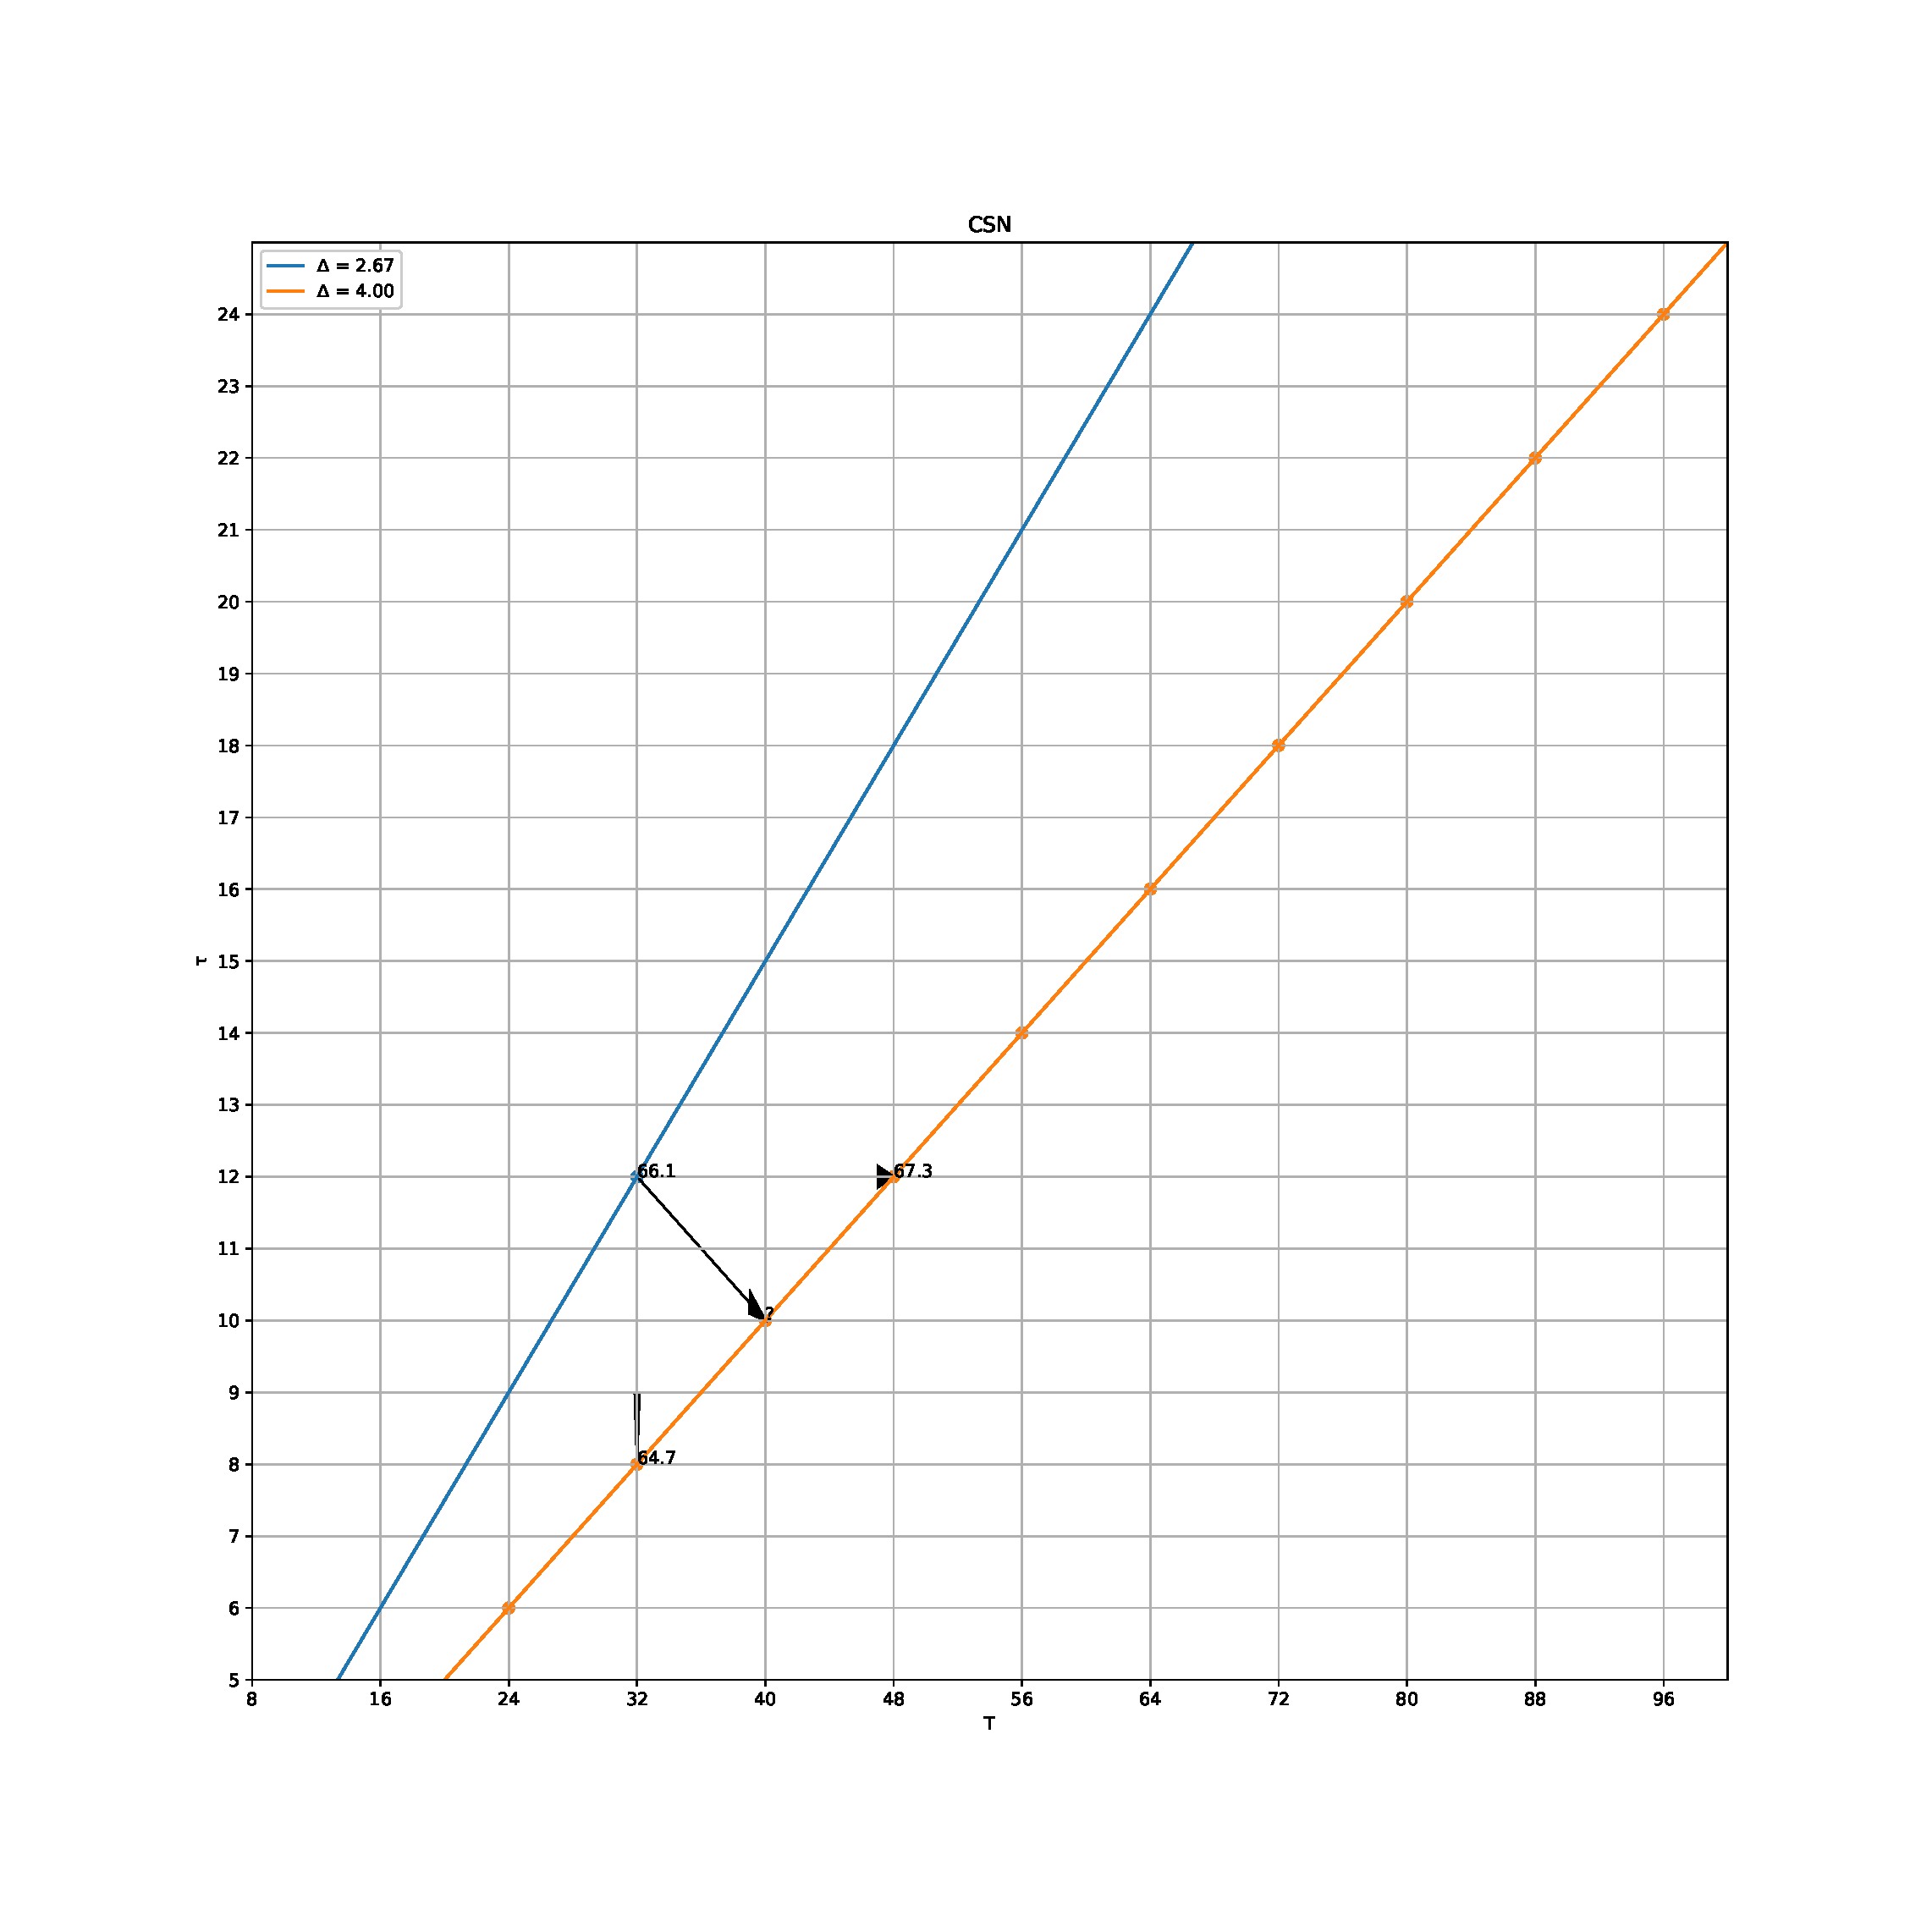
\includegraphics[width=0.99\textwidth, keepaspectratio, interpolate]{img/07_grid_csn.eps}
        \caption{Punkte für Grid-Suche}
        \label{fig:exp-hparams-grid}
    \end{subfigure}%
    \begin{subfigure}{.35\textwidth}
        \centering
        \includegraphics[width=0.99\textwidth, keepaspectratio, interpolate]{img/07_par_cor_prec.eps}
        \caption{Precision für Grid-Suche}
        \label{fig:exp-hparams-prec}
    \end{subfigure}
    \begin{subfigure}{.35\textwidth}
        \centering
        \includegraphics[width=0.99\textwidth, keepaspectratio, interpolate]{img/07_par_cor_rec.eps}
        \caption{Recall für Grid-Suche}
        \label{fig:exp-hparams-rec}
    \end{subfigure}
\end{figure}

Aufgrund der Vielzahl zusätzlicher Experimente wird die Laufzeit bei diesen Experimenten durch $\gls{tld:Theta}_\text{train} = 100$ und auf 3 Epochen begrenzt.
Da das Baseline-Modell nach der ersten Phase bereits neue Feature gelernt hat, wird zu Beginn eine neue Lernrate gesucht, die für alle Trainings der Grid-Suche gilt und dem Intervall $[3e^{-4}, 3e^{-6}]$ entspricht.
\autoref{fig:exp-hparams-prec} und \autoref{fig:exp-hparams-rec} veranschaulichen die Ergebnisse der Grid-Suche in Form von Parallelen Koordinaten.
Es fällt auf, dass die Hyperparameter sehr gegensätzlichen Einfluss auf die Metriken Precision und Recall haben.
So wirken sich zusätzliche Frames und ein hoher oder gleichbleibender Zeitschritt positiv auf den Recall aus, während sich beides eher negativ auf die Precision auswirkt.
Ein erhöhter Zeitkontext wirkt sich ebenfalls positiv auf den Recall auf.
Die Precision scheint hingegen unabhängig vom Zeitkontext zu sein.

Um ein gutes Gleichgewicht zwischen den beiden Metriken zu erlangen, werden nachfolgend nur noch Ergebnisse betrachtet, die einen besonders hohen F1-Score aufweisen.
In \autoref{tab:phase2} sind diese Experimente gelistet, die maximal 1 \% von dem maximale F1-Score abweichen.
Als zusätzlicher Filter werden Experimente ausgeschlossen, deren Balanced Accuracy mehr als 1 \% vom Maximum abweicht.

\begin{figure}
    \centering
    \small
    \csvreader[no head,tabular=|r|r|r||r|r|r|,
    table head=\hline,late after line=\\\hline]{tbl/exp_phase_2.csv}
    {1=\model,2=\s,3=\t,4=\sr,5=\d,6=\auroc,7=\ba,8=\fone}
    {\t & \sr & \d & \ba & \fone & \auroc}
    \caption{Ergebnisse aus Phase 2}
    \label{tab:phase2}
\end{figure}


Das jeweils beste Modell wird nach Abschluss der Suche erneut für 5 Epochen mit $\gls{tld:Theta}_\text{train} = 200$ trainiert.

\section{Kategorisierung der Aktionsklassen}
\label{sec:kategorisierung-der-aktionsklassen}

\begin{tcolorbox}[title=Todo]
    \begin{itemize}
        \item Abweichung pro Metrik erheben: Klasse zu macro -> Durchschnitt
        \item Idee: pca und clustering in vier gruppen
        \item Vergleich der Evaluation auf subsets (SOCC-HAR-8, -16, -24, -32): Jeweils ROC Curve
        \item Optional: SOCC-HAR-NET, SOCC-HAR-DB Klassen
    \end{itemize}
\end{tcolorbox}

\begin{figure}
    \centering
    \begin{subfigure}{.24\textwidth}
        \centering
        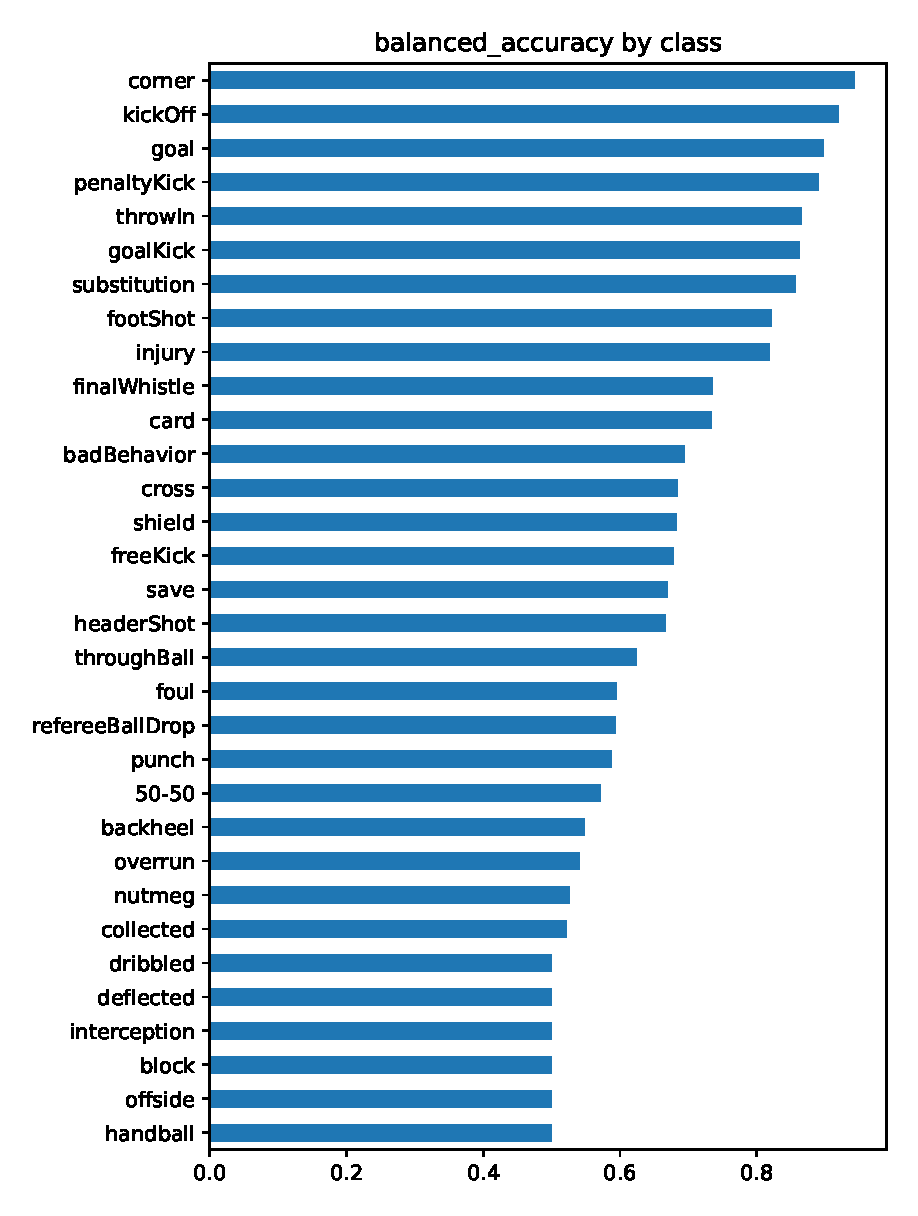
\includegraphics[width=0.99\textwidth, keepaspectratio, interpolate]{img/07_balanced_accuracy_by_class_test_202012-2218-2841.eps}
    \end{subfigure}%
    \begin{subfigure}{.24\textwidth}
        \centering
        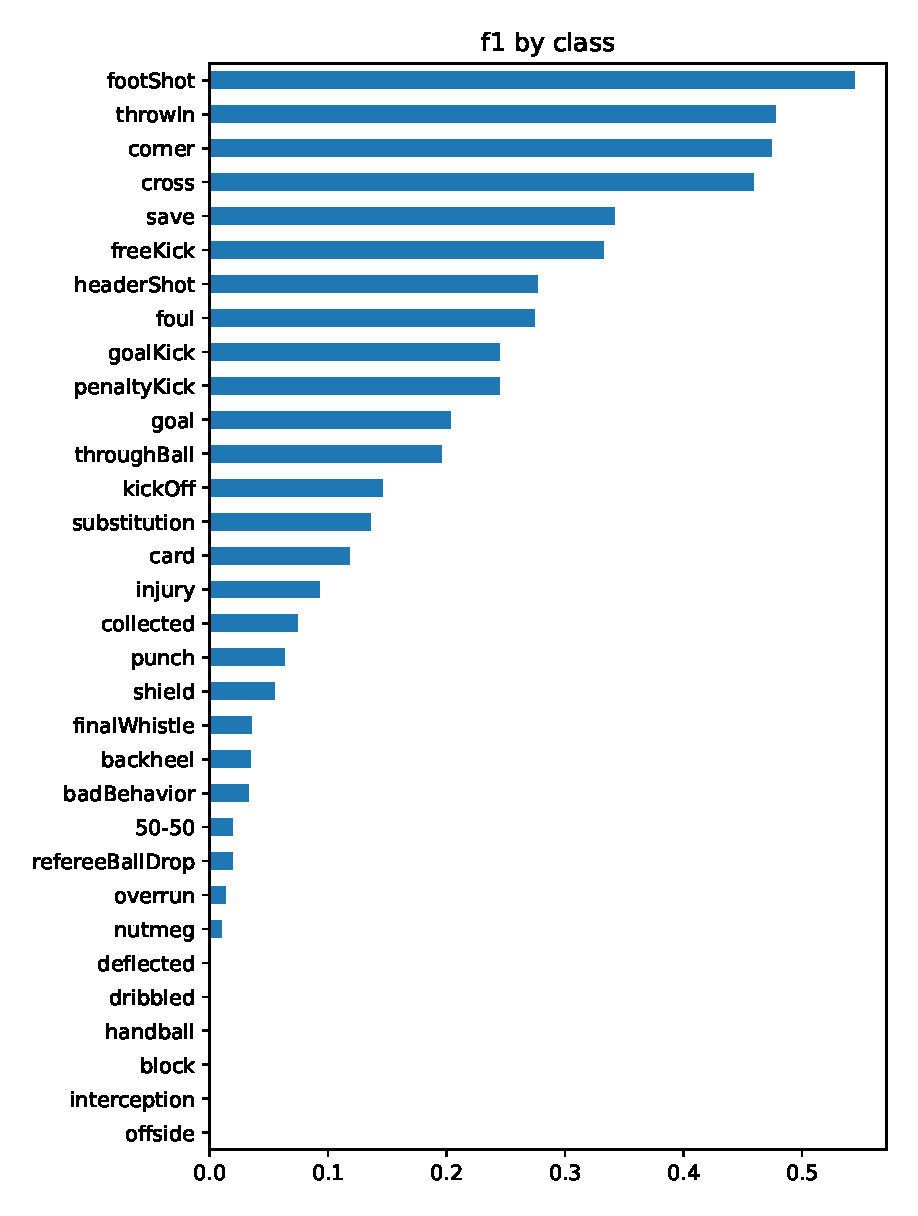
\includegraphics[width=0.99\textwidth, keepaspectratio, interpolate]{img/07_f1_by_class_test_202012-2218-2841.eps}
    \end{subfigure}
    \begin{subfigure}{.24\textwidth}
        \centering
        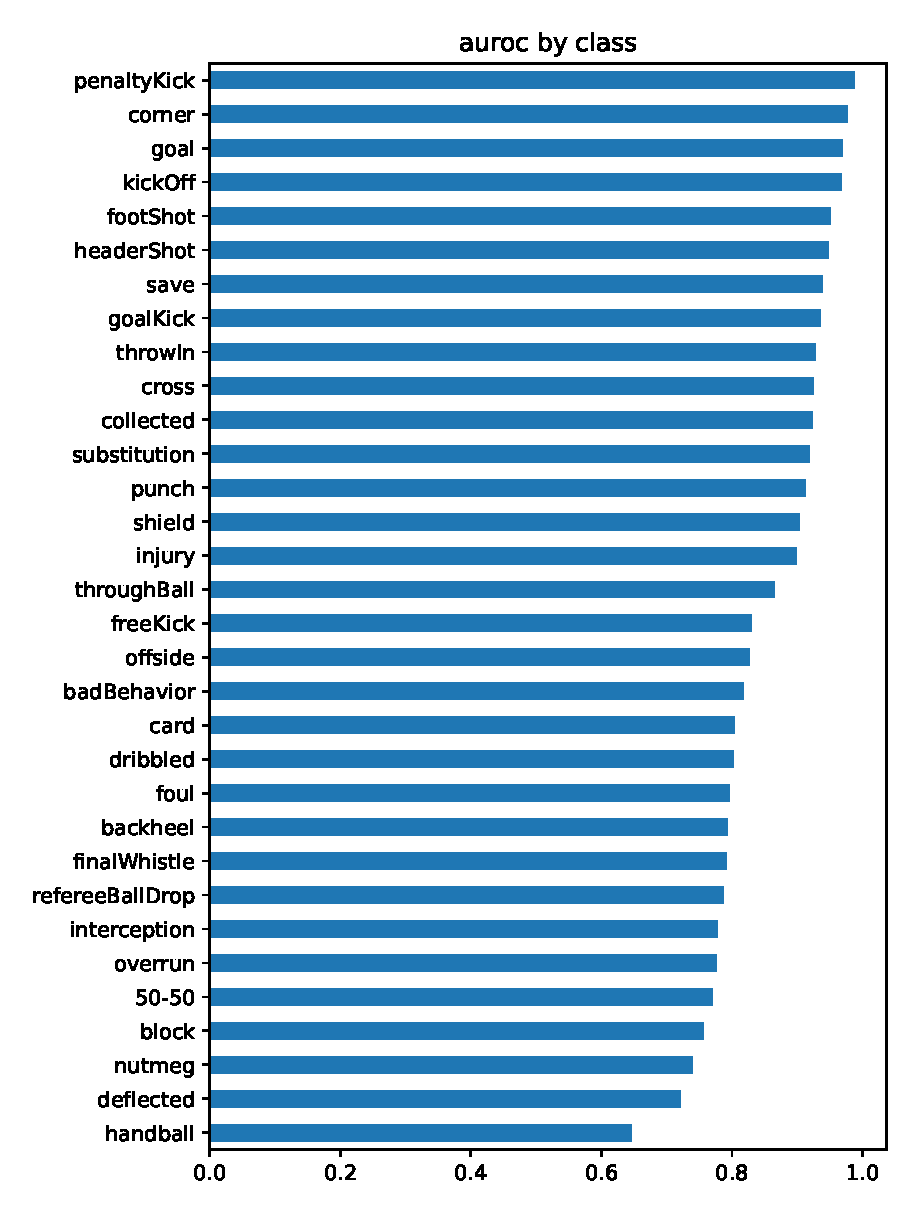
\includegraphics[width=0.99\textwidth, keepaspectratio, interpolate]{img/07_auroc_by_class_test_202012-2218-2842.eps}
    \end{subfigure}
    \begin{subfigure}{.24\textwidth}
        \centering
        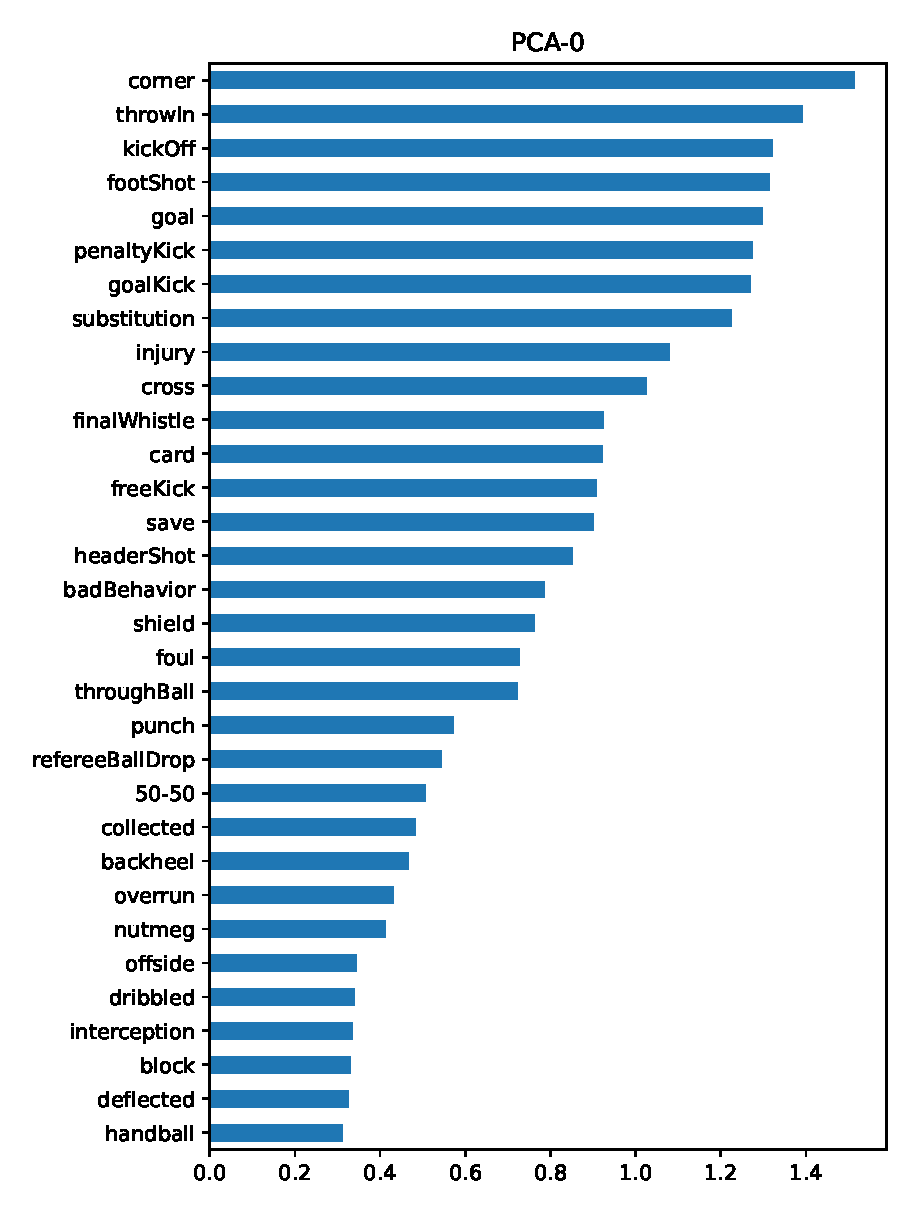
\includegraphics[width=0.99\textwidth, keepaspectratio, interpolate]{img/07_PCA_by_class_test_202012-2218-2843.eps}
    \end{subfigure}
    \caption{Metriken pro Klasse}
    \label{fig:class-metrics}
\end{figure}

Die bisherigen Rechenergebnissen wurden jeweils die durchschnittlichen Metriken (macro) über alle Klassen betrachtet.
In diesem Abschnitt wird das Top-Modell hingegen an jeder Klasse einzeln evaluiert.
Dazu werden die bereits verwendeten Metriken pro Klasse erhoben.
Wie \autoref{fig:class-metrics} zu entnehmen ist, gibt es starke Abweichungen innerhalb der verschiedenen Klassen.
Während Aktionen wie \code{corner}, \code{footShot} oder \code{throwIn} durchgehend hohe Metriken vorweisen, können andere Klassen wie \code{offside} oder \code{handball} praktisch gar nicht klassifizieren werden.
Zwischen diesen Extrema ist es schwierig eine klare Rangordnung von leicht zu schwierig herzustellen.
Das wird insbesondere deutlich wenn man die Metriken Precision und Recall in \autoref{fig:precision-recall} betrachtet.

\begin{figure}
    \centering
    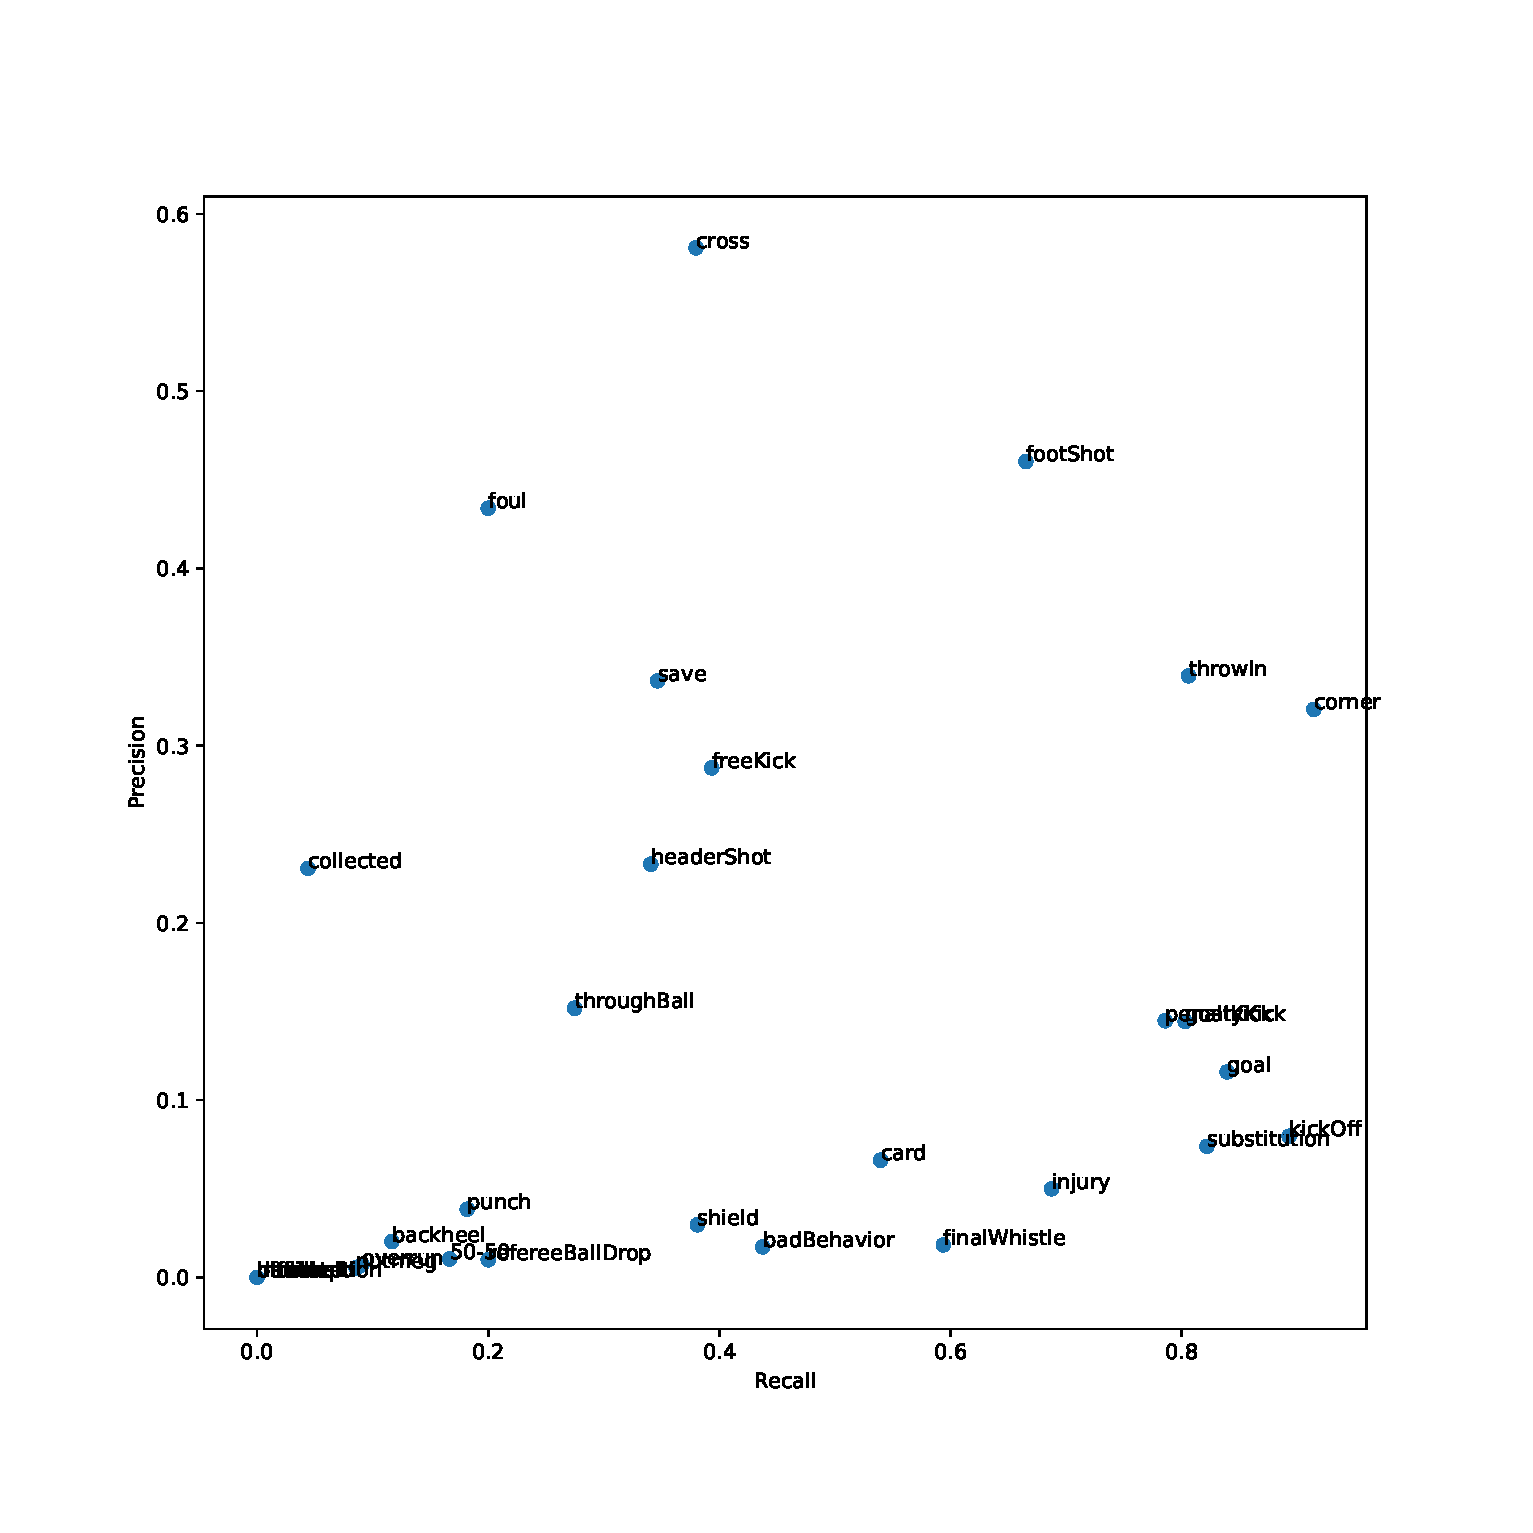
\includegraphics[width=0.99\textwidth, keepaspectratio, interpolate]{img/07_precision_recall_by_class.eps}
    \caption{Vergleich von Precision und Recall pro Klasse}
    \label{fig:precision-recall}
\end{figure}

Dabei fällt auch auf, dass vor die Klassen im unteren Bereich mit einer niedrigen Precision viele False Positives verursachen, obwohl sie zum Teil einen hohen Recall haben.
Auffällig ist auch, dass Aktionen, die sich im laufenden Spiel ereignen (\code{foul}, \code{cross}, \code{footShot}, \code{save}) einen besonders hohen Recall haben, während Aktionen die oft mit Spielunterbrechungen und Nahaufnahmen einhergehen (\code{substitution}, \code{goal}, \code{injury}) einen sehr niedrigen Recall aufweisen.

Man sieht also, dass keine pauschale Aussage über die Schwierigkeit der Aktionsklassen gemacht werden kann.
Dennoch lässt sich anhand der erfassten Metriken eine grobe Ordnung erstellen, auch wenn sie allgemein nicht repräsentativ ist.
Hierzu werden alle Metriken pro Klasse zu einer zweidimensionalen Matrix $M \in (A \times 5)$ gesammelt und im Zuge einer \gls{pca} auf einen eindimensionalen Vektor projiziert.
Die erste Komponente der \gls{pca} $c_0 \in (5 \times 1)$ deckt mit 80 \% hinreichend viel Varianz und projiziert die Metriken auf einen Vektor:

\begin{equation}
    \label{eq:pca}
    \text{pca}_0 = M \cdot c_0
\end{equation}

Die resultierende Rangordnung ist ebenfalls in \autoref{fig:class-metrics} (rechts) abgebildet.

\subsection{Evaluation auf Teilmengen}
\label{subsec:evaluation-auf-teilmengen}

Abschließend soll der Einfluss schwächerer Klassen auf das Gesamtergebnis gemessen werden.
Dazu werden die Aktionsklassen absteigend nach der PCA-basierten Rangordnung sortiert und in vier Teilmengen gegliedert, die sich jeweils aus den oberen 8, 16, 24 und 32 Klassen zusammensetzen.
In \autoref{tab:eval_subset} sind die Ergebnisse (macro) auf Berechnungsgrundlage der in der jeweiligen Teilmenge enthaltenen Klassen aufgeführt.
Zusätzlich wurden zwei weitere Untermengen mit den gleichen Aktionsklassen aus den Datensets SoccerNet und SoccerDB abgeleitet.
Die Ergebnisse sind keinesfalls direkt vergleichbar mit den publizierten Datensets, da die Datengrundlage eine andere ist.
Es soll dem Leser jedoch eine grobe Einordnung ermöglichen.

\begin{figure}
    \centering
    \csvreader[no head,tabular=|l||r|r|r|,
    table head=\hline,late after line=\\\hline]{tbl/eval_subsets.csv}
    {1=\dataset,2=\ba,3=\fbeta,4=\auroc}
    {\dataset & \ba & \fbeta & \auroc}
    \caption{Evaluation auf Teilmengen von Aktionsklassen}
    \label{tab:eval_subset}
\end{figure}

\section{Fine-Tuning}

\begin{tcolorbox}[title=WIP]
    \begin{itemize}
        \item Tabelle: Label Smooting, res,Anzahl Epochen, Weight Decay
        \item Mit mehr Background trainieren um Precision zu erhöhen!
        \item schon hier beschränken auf 24 Klassen?
        \item Threshold auf Validierungsset bestimmen und an Testset testen
    \end{itemize}
\end{tcolorbox}

In der vierten Phase wird das neue Baseline-Modell aus Phase 3 mit zusätzlichen Techniken weiter optimiert.
Dazu zählt das Training mit einer erhöhten Auflösung $S$, der Einsatz von Label Smoothing \cite{Szegedy15} und die Justierung weitere Hyperparameter wie Weight Decay.
\autoref{tab:exp4} zeigt die Ergebnisse.

\begin{figure}
    \centering
    \csvreader[no head,tabular=|l|r||r|r|r||r|r|r|,
    table head=\hline,late after line=\\\hline]{tbl/exp_phase_4.csv}
    {1=\model,2=\wdecay,3=\s,4=\thet,5=\auroc,6=\ba,7=\fbeta,8=\epo}
    {\model & \s & \epo & \thet & \wdecay & \ba & \fbeta & \auroc}
    \caption{Ergebnisse aus Phase 4}
    \label{tab:exp4}
\end{figure}